% Define block styles
\tikzstyle{block} = [draw, rectangle, fill=white, minimum height=3cm, minimum width=3.9cm, text width=3.7cm, text centered, rounded corners=true]
\tikzstyle{blockBox} = [draw, inner sep=0.2cm, dashed, rectangle, minimum width=3.5cm, text centered, rounded corners=true]
\tikzstyle{blockText} = [text centered, minimum height=1.5cm,text width=3.9cm]
\tikzstyle{blockS} = [text centered, text width=1.1cm, minimum height=0.5cm, rounded corners=true, fill=white]
\tikzstyle{arrow} = [draw, -latex]

\definecolor{red1}{RGB}{160,0,0}
\definecolor{green1}{RGB}{0,160,0}
\definecolor{blue1}{RGB}{0,0,160}

% Define images
\pgfdeclareimage[height=2.8cm]{scene}{./figures/perception/methods/visualodometryalgorithm/flowchart_scene.jpg}
\pgfdeclareimage[height=2.8cm]{features}{./figures/perception/methods/visualodometryalgorithm/flowchart_features_frame.jpg}
\pgfdeclareimage[width=3.6cm]{transform}{./figures/perception/methods/visualodometryalgorithm/flowchart_transform.jpg}
\pgfdeclareimage[height=2.4cm]{triangulation}{./figures/perception/methods/visualodometryalgorithm/flowchart_triangulation.png}
\pgfdeclareimage[height=2.8cm]{pointcloud}{./figures/perception/methods/visualodometryalgorithm/flowchart_pointcloud_small.jpg}

\newsavebox\mybox
\begin{lrbox}{\mybox}
  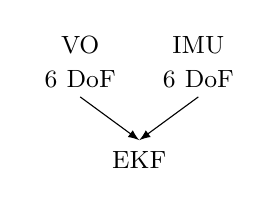
\begin{tikzpicture}[node distance=1.5cm, auto]
    \node [blockS] (s1) {\small{VO\\6~DoF}};
    \node [blockS, right of=s1] (s2) {\small{IMU\\6~DoF}};
    %\node [blockS, below of=s1, node distance=1cm] (s4) {\pgfuseimage{picRottrans}};
    \node [blockS, below of=s1, xshift=0.75cm, node distance=1.25cm, text width=2.5cm] (s3) {\small{EKF}};

    \draw [arrow] (s1.south) to (s3.north);
    \draw [arrow] (s2.south) to (s3.north);
  \end{tikzpicture}
\end{lrbox}

	      
\begin{tikzpicture}[node distance = 5.0cm, auto]
  % Scene
  \node[block] (scene) {\pgfuseimage{scene}};

	% Features and Optical flow
  \node [block, right of=scene] (features) {\pgfuseimage{features}};

  % Transform
  \node [block, right of=features] (transform) {\pgfuseimage{transform}};
  

  % EKF
  \node [block, below of=scene, node distance=6.0cm] (ekf) {\usebox\mybox};
  
  % Depth
  \node [block, right of=ekf] (triangulation) {\pgfuseimage{triangulation}};
  
  % Point Cloud
  \node [block, right of=triangulation] (pointcloud) {\pgfuseimage{pointcloud}};
  
  
  % Text
  \node [blockText, above of=scene, node distance=2.2cm] (scene_t) {\textbf{a) Scene}};
  \node [blockText, above of=features, node distance=2.2cm] (features_t) {\textbf{b) Features and optical flow}};
  \node [blockText, above of=transform, node distance=2.2cm] (transform_t) {\textbf{c) Dewarp}};
  \node [blockText, above of=ekf, node distance=2.2cm] (ekf_t) {\textbf{d) Fuse}};
  \node [blockText, above of=triangulation, node distance=2.2cm] (triangulation_t) {\textbf{e) Compute depth}};
  \node [blockText, above of=pointcloud, node distance=2.2cm] (pointcloud_t) {\textbf{f) Generate point cloud}};


  % Fit
  \node[fit=(scene)(scene_t), blockBox] (scene_f) {};
  \node[fit=(features)(features_t), blockBox] (features_f) {};
  \node[fit=(transform)(transform_t), blockBox] (tranform_f) {};
  \node[fit=(ekf)(ekf_t), blockBox] (ekf_f) {};
  \node[fit=(triangulation)(triangulation_t), blockBox] (triangulation_f) {};
  \node[fit=(pointcloud)(pointcloud_t), blockBox] (pointcloud_f) {};


  % Arrows
	\path [arrow] (scene_f.east) to (features_f.west);
	\path [arrow] (features_f.east) to (tranform_f.west);
	\path [arrow] (tranform_f.south) -| ++(0,-0.55cm) -| (ekf_f.north);
	\path [arrow] (ekf_f.east) to (triangulation_f.west);
	\path [arrow] (triangulation_f.east) to (pointcloud_f.west);
\end{tikzpicture}
